\documentclass[12pt,letterpaper]{article}
\usepackage{graphicx,textcomp}
\usepackage{natbib}
\usepackage{setspace}
\usepackage{fullpage}
\usepackage{color}
\usepackage[reqno]{amsmath}
\usepackage{amsthm}
\usepackage{fancyvrb}
\usepackage{amssymb,enumerate}
\usepackage[all]{xy}
\usepackage{endnotes}
\usepackage{lscape}
\newtheorem{com}{Comment}
\usepackage{float}
\usepackage{hyperref}
\newtheorem{lem} {Lemma}
\newtheorem{prop}{Proposition}
\newtheorem{thm}{Theorem}
\newtheorem{defn}{Definition}
\newtheorem{cor}{Corollary}
\newtheorem{obs}{Observation}
\usepackage[compact]{titlesec}
\usepackage{dcolumn}
\usepackage{tikz}
\usetikzlibrary{arrows}
\usepackage{multirow}
\usepackage{xcolor}
\newcolumntype{.}{D{.}{.}{-1}}
\newcolumntype{d}[1]{D{.}{.}{#1}}
\definecolor{light-gray}{gray}{0.65}
\usepackage{url}
\usepackage{listings}
\usepackage{color}

\definecolor{codegreen}{rgb}{0,0.6,0}
\definecolor{codegray}{rgb}{0.5,0.5,0.5}
\definecolor{codepurple}{rgb}{0.58,0,0.82}
\definecolor{backcolour}{rgb}{0.95,0.95,0.92}

\lstdefinestyle{mystyle}{
	backgroundcolor=\color{backcolour},   
	commentstyle=\color{codegreen},
	keywordstyle=\color{magenta},
	numberstyle=\tiny\color{codegray},
	stringstyle=\color{codepurple},
	basicstyle=\footnotesize,
	breakatwhitespace=false,         
	breaklines=true,                 
	captionpos=b,                    
	keepspaces=true,                 
	numbers=left,                    
	numbersep=5pt,                  
	showspaces=false,                
	showstringspaces=false,
	showtabs=false,                  
	tabsize=2
}
\lstset{style=mystyle}
\newcommand{\Sref}[1]{Section~\ref{#1}}
\newtheorem{hyp}{Hypothesis}

\title{Problem Set 3}
\date{Due: November 13, 2025}
\author{Applied Stats/Quant Methods 1}


\begin{document}
	\maketitle
	\section*{Instructions}
	\begin{itemize}
		\item Please show your work! You may lose points by simply writing in the answer. If the problem requires you to execute commands in \texttt{R}, please include the code you used to get your answers. Please also include the \texttt{.R} file that contains your code. If you are not sure if work needs to be shown for a particular problem, please ask.
	\item Your homework should be submitted electronically on GitHub.
	\item This problem set is due before 23:59 on Thursday November 13, 2025. No late assignments will be accepted.

	\end{itemize}

		\vspace{.25cm}
	
\noindent In this problem set, you will run several regressions and create an add variable plot (see the lecture slides) in \texttt{R} using the \texttt{incumbents\_subset.csv} dataset. Include all of your code.

	\vspace{.5cm}
\section*{Question 1}
\vspace{.25cm}
\noindent We are interested in knowing how the difference in campaign spending between incumbent and challenger affects the incumbent's vote share. 
	\begin{enumerate}
		\item Run a regression where the outcome variable is \texttt{voteshare} and the explanatory variable is \texttt{difflog}.	\vspace{5cm}
	\begin{table}[!htbp] \centering 
		\caption{Regression Results for Model 1: voteshare ~ difflog} 
		\label{} 
		\begin{tabular}{@{\extracolsep{5pt}}lD{.}{.}{-4} } 
			\\[-1.8ex]\hline 
			\hline \\[-1.8ex] 
			& \multicolumn{1}{c}{\textit{Dependent variable:}} \\ 
			\cline{2-2} 
			\\[-1.8ex] & \multicolumn{1}{c}{Incumbent Vote Share} \\ 
			\hline \\[-1.8ex] 
			Spending Difference (difflog) & 0.0417^{***} \\ 
			& (0.0010) \\ 
			Constant & 0.5790^{***} \\ 
			& (0.0023) \\ 
			\hline \\[-1.8ex] 
			Observations & \multicolumn{1}{c}{3,193} \\ 
			R$^{2}$ & \multicolumn{1}{c}{0.3673} \\ 
			Adjusted R$^{2}$ & \multicolumn{1}{c}{0.3671} \\ 
			\hline 
			\hline \\[-1.8ex] 
			\textit{Note:}  & \multicolumn{1}{r}{$^{*}$p$<$0.1; $^{**}$p$<$0.05; $^{***}$p$<$0.01} \\ 
		\end{tabular} 
	\end{table}                    
		\lstinputlisting[language=R, firstline=33, lastline=48]{PS03_RS.R}  
		\item Make a scatterplot of the two variables and add the regression line. 	\vspace{0.5cm}
		\lstinputlisting[language=R, firstline=51, lastline=61]{PS03_RS.R}  
		{\centering
			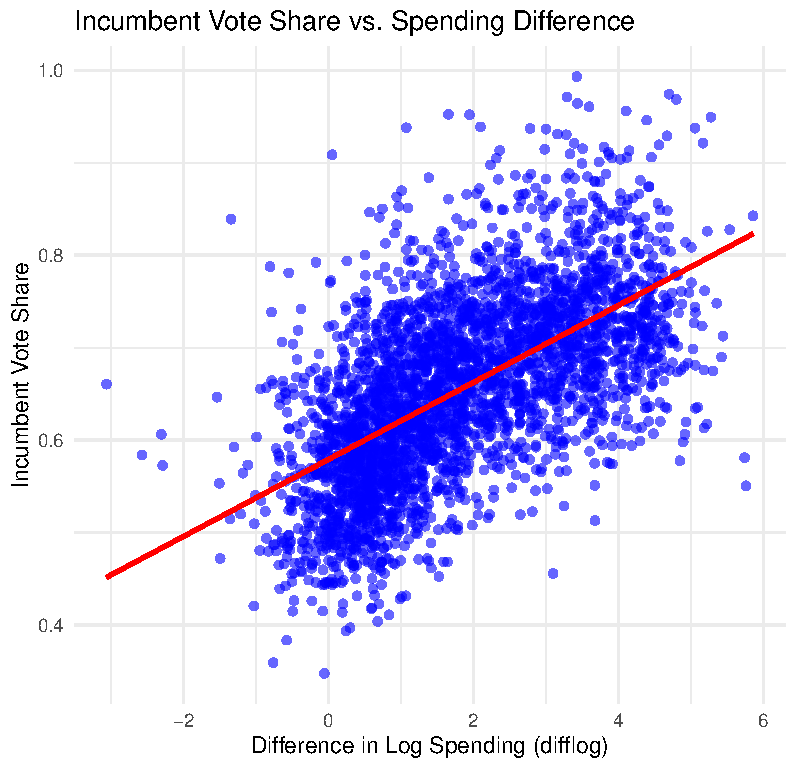
\includegraphics[width=\textwidth]{plot1.pdf}\par}
		\item Save the residuals of the model in a separate object.	\vspace{0.5cm}
			\lstinputlisting[language=R, firstline=63, lastline=65]{PS03_RS.R}  
		\item Write the prediction equation.
		\lstinputlisting[language=R, firstline=67, lastline=68]{PS03_RS.R}  
		\textbf{$\widehat{voteshare}$ = 0.58 + 0.04 x difflog}
	\end{enumerate}
	
\newpage

\section*{Question 2}
\noindent We are interested in knowing how the difference between incumbent and challenger's spending and the vote share of the presidential candidate of the incumbent's party are related.	\vspace{.25cm}
	\begin{enumerate}
		\item Run a regression where the outcome variable is \texttt{presvote} and the explanatory variable is \texttt{difflog}.	\vspace{0.5cm}
		\lstinputlisting[language=R, firstline=70, lastline=81]{PS03_RS.R}  
	\begin{table}[!htbp] \centering 
		\caption{Regression Results for Model 2: presvote ~ difflog} 
		\label{} 
		\begin{tabular}{@{\extracolsep{5pt}}lD{.}{.}{-4} } 
			\\[-1.8ex]\hline 
			\hline \\[-1.8ex] 
			& \multicolumn{1}{c}{\textit{Dependent variable:}} \\ 
			\cline{2-2} 
			\\[-1.8ex] & \multicolumn{1}{c}{presvote} \\ 
			\hline \\[-1.8ex] 
			Spending Difference (difflog) & 0.0238^{***} \\ 
			& (0.0014) \\ 
			Constant & 0.5076^{***} \\ 
			& (0.0032) \\ 
			\hline \\[-1.8ex] 
			Observations & \multicolumn{1}{c}{3,193} \\ 
			R$^{2}$ & \multicolumn{1}{c}{0.0880} \\ 
			Adjusted R$^{2}$ & \multicolumn{1}{c}{0.0877} \\ 
			\hline 
			\hline \\[-1.8ex] 
			\textit{Note:}  & \multicolumn{1}{r}{$^{*}$p$<$0.1; $^{**}$p$<$0.05; $^{***}$p$<$0.01} \\ 
		\end{tabular} 
	\end{table} 
		\item Make a scatterplot of the two variables and add the regression line. 	\vspace{0.5cm}
				\lstinputlisting[language=R, firstline=83, lastline=92]{PS03_RS.R}  
		{\centering
			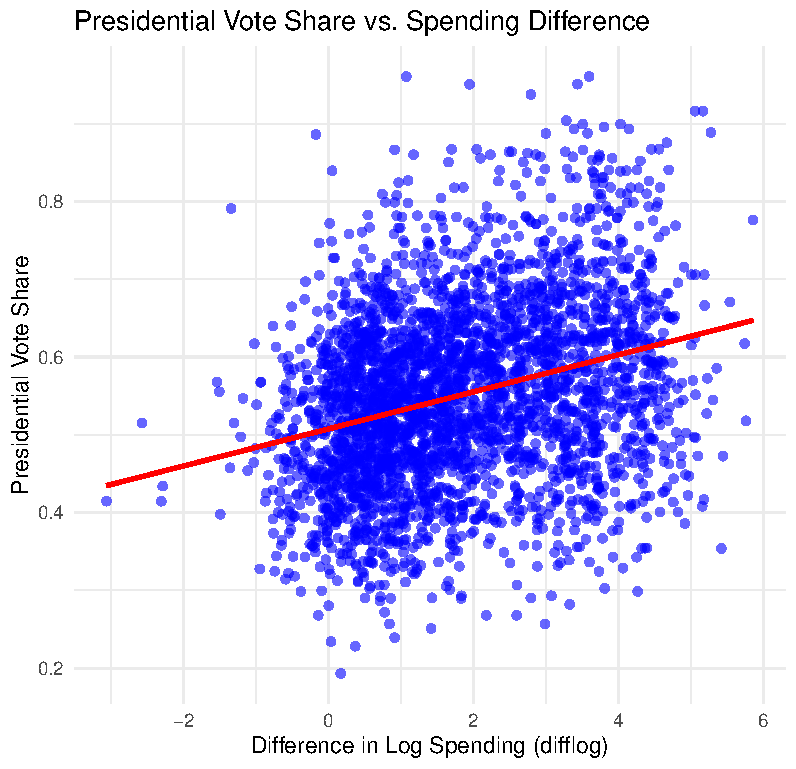
\includegraphics[width=\textwidth]{plot2.pdf}\par}
		\item Save the residuals of the model in a separate object.	\vspace{0.5cm}
				\lstinputlisting[language=R, firstline=94, lastline=96]{PS03_RS.R}  
		\item Write the prediction equation.
		       \lstinputlisting[language=R, firstline=98, lastline=99]{PS03_RS.R}  
		\textbf{{$\widehat{presvote}$.} = 0.51 + 0.02 x difflog} 
	\end{enumerate}
	
	\newpage	
\section*{Question 3}

\noindent We are interested in knowing how the vote share of the presidential candidate of the incumbent's party is associated with the incumbent's electoral success.
	\vspace{.25cm}
	\begin{enumerate}
		\item Run a regression where the outcome variable is \texttt{voteshare} and the explanatory variable is \texttt{presvote}.
			\vspace{0.5cm}
					\lstinputlisting[language=R, firstline=101, lastline=112]{PS03_RS.R}  
					\begin{table}[!htbp] \centering 
						\caption{Regression Results for Model 3: voteshare ~ presvote} 
						\label{} 
						\begin{tabular}{@{\extracolsep{5pt}}lD{.}{.}{-4} } 
							\\[-1.8ex]\hline 
							\hline \\[-1.8ex] 
							& \multicolumn{1}{c}{\textit{Dependent variable:}} \\ 
							\cline{2-2} 
							\\[-1.8ex] & \multicolumn{1}{c}{Incumbent Vote Share} \\ 
							\hline \\[-1.8ex] 
							presvote & 0.3880^{***} \\ 
							& (0.0135) \\ 
							Constant & 0.4413^{***} \\ 
							& (0.0076) \\ 
							\hline \\[-1.8ex] 
							Observations & \multicolumn{1}{c}{3,193} \\ 
							R$^{2}$ & \multicolumn{1}{c}{0.2058} \\ 
							Adjusted R$^{2}$ & \multicolumn{1}{c}{0.2056} \\ 
							\hline 
							\hline \\[-1.8ex] 
							\textit{Note:}  & \multicolumn{1}{r}{$^{*}$p$<$0.1; $^{**}$p$<$0.05; $^{***}$p$<$0.01} \\ 
						\end{tabular} 
					\end{table} 
		\item Make a scatterplot of the two variables and add the regression line. 
			\vspace{0.5cm}
			\lstinputlisting[language=R, firstline=114, lastline=123]{PS03_RS.R}  
				{\centering
				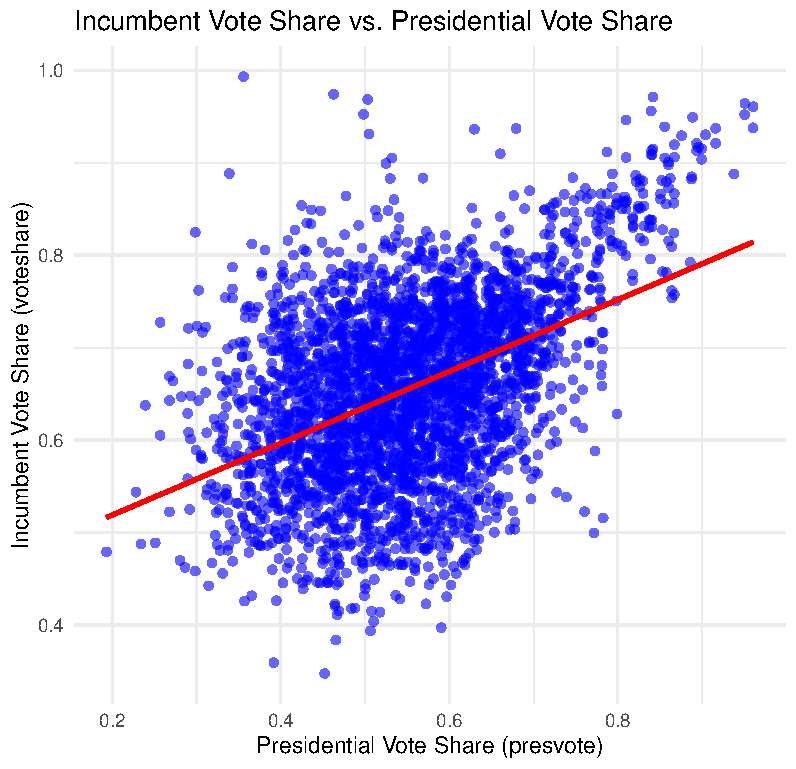
\includegraphics[width=\textwidth]{plot3.pdf}\par}
		\item Write the prediction equation.
		\lstinputlisting[language=R, firstline=125, lastline=126]{PS03_RS.R}  
		\textbf{{$\widehat{voteshare}$} = 0.44 + 0.39 x presvote}
	\end{enumerate}
	

\newpage	
\section*{Question 4}
\noindent The residuals from part (a) tell us how much of the variation in \texttt{voteshare} is $not$ explained by the difference in spending between incumbent and challenger. The residuals in part (b) tell us how much of the variation in \texttt{presvote} is $not$ explained by the difference in spending between incumbent and challenger in the district.
	\begin{enumerate}
		\item Run a regression where the outcome variable is the residuals from Question 1 and the explanatory variable is the residuals from Question 2.	\vspace{0.5cm}
			\lstinputlisting[language=R, firstline=128, lastline=139]{PS03_RS.R}  
\begin{table}[!htbp] \centering 
	\caption{Regression Results for Model 4: residual model ~ residuals model2} 
	\label{} 
	\begin{tabular}{@{\extracolsep{5pt}}lD{.}{.}{-4} } 
		\\[-1.8ex]\hline 
		\hline \\[-1.8ex] 
		& \multicolumn{1}{c}{\textit{Dependent variable:}} \\ 
		\cline{2-2} 
		\\[-1.8ex] & \multicolumn{1}{c}{residual model} \\ 
		\hline \\[-1.8ex] 
		residual model2 & 0.2569^{***} \\ 
		& (0.0118) \\ 
		Constant & -0.0000 \\ 
		& (0.0013) \\ 
		\hline \\[-1.8ex] 
		Observations & \multicolumn{1}{c}{3,193} \\ 
		R$^{2}$ & \multicolumn{1}{c}{0.1300} \\ 
		Adjusted R$^{2}$ & \multicolumn{1}{c}{0.1298} \\ 
		\hline 
		\hline \\[-1.8ex] 
		\textit{Note:}  & \multicolumn{1}{r}{$^{*}$p$<$0.1; $^{**}$p$<$0.05; $^{***}$p$<$0.01} \\ 
	\end{tabular} 
\end{table} 
		\item Make a scatterplot of the two residuals and add the regression line. 	\vspace{6cm}
		\lstinputlisting[language=R, firstline=141, lastline=150]{PS03_RS.R}  
		{\centering
		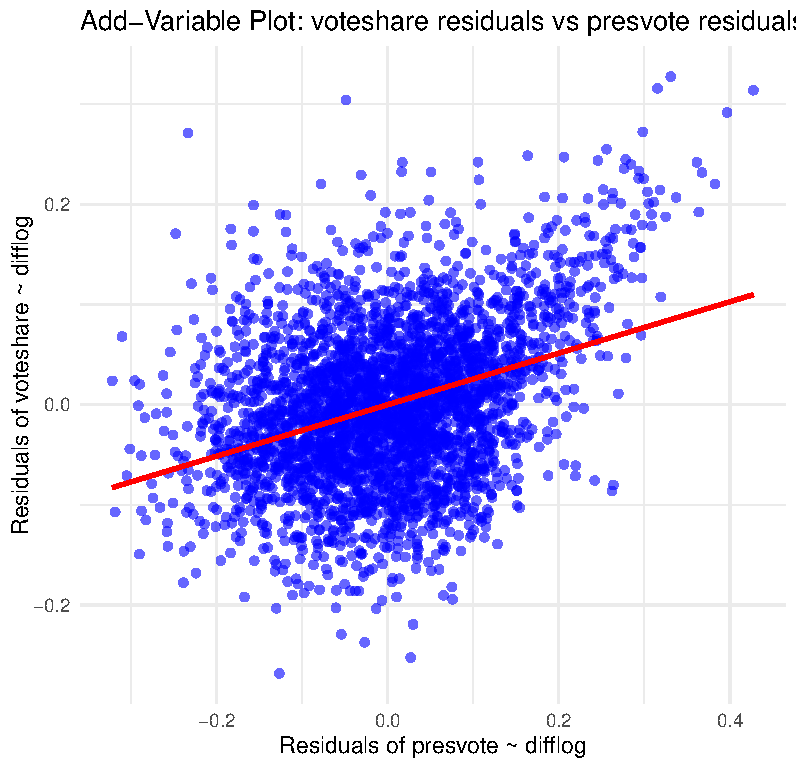
\includegraphics[width=\textwidth]{plot4.pdf}\par}
		\item Write the prediction equation.
		\lstinputlisting[language=R, firstline=152, lastline=154]{PS03_RS.R}  
		\textbf{$\widehat{residual model}$ = 0 + 0.26 x residucal model2 }
	\end{enumerate}
	
	\newpage	

\section*{Question 5}
\noindent What if the incumbent's vote share is affected by both the president's popularity and the difference in spending between incumbent and challenger? 
	\begin{enumerate}
		\item Run a regression where the outcome variable is the incumbent's \texttt{voteshare} and the explanatory variables are \texttt{difflog} and \texttt{presvote}.	\vspace{0.5cm}
		\lstinputlisting[language=R, firstline=156, lastline=167]{PS03_RS.R}  
		\begin{table}[!htbp] \centering 
			\caption{Regression Results for Model 4: voteshare ~ difflog + presvote} 
			\label{} 
			\begin{tabular}{@{\extracolsep{5pt}}lD{.}{.}{-4} } 
				\\[-1.8ex]\hline 
				\hline \\[-1.8ex] 
				& \multicolumn{1}{c}{\textit{Dependent variable:}} \\ 
				\cline{2-2} 
				\\[-1.8ex] & \multicolumn{1}{c}{Incumbent Vote Share} \\ 
				\hline \\[-1.8ex] 
				Spending Difference (difflog) + presvote & 0.0355^{***} \\ 
				& (0.0009) \\ 
				presvote & 0.2569^{***} \\ 
				& (0.0118) \\ 
				Constant & 0.4486^{***} \\ 
				& (0.0063) \\ 
				\hline \\[-1.8ex] 
				Observations & \multicolumn{1}{c}{3,193} \\ 
				R$^{2}$ & \multicolumn{1}{c}{0.4496} \\ 
				Adjusted R$^{2}$ & \multicolumn{1}{c}{0.4493} \\ 
				\hline 
				\hline \\[-1.8ex] 
				\textit{Note:}  & \multicolumn{1}{r}{$^{*}$p$<$0.1; $^{**}$p$<$0.05; $^{***}$p$<$0.01} \\ 
			\end{tabular} 
		\end{table} 
		\item Write the prediction equation.	\vspace{5cm}
		\lstinputlisting[language=R, firstline=169, lastline=1707]{PS03_RS.R}  
		\textbf{{$\widehat{voteshare}$} = 0.49 + 0.036 x difflog + 0.26 x presvote}
		\item What is it in this output that is identical to the output in Question 4? Why do you think this is the case?
	
		\textbf{The idenntical value in question 4 and 5 is the coefficient of presvote (0.26). This is because the effect of presvote on voteshare, controlling for difflog, is the same whether you include difflog directly in a multiple regression or “remove” its influence first and then regress the residuals. }
	\end{enumerate}




\end{document}
